% RSS 2027 Stage 1 extended abstract (5 pages of content + 1 page of references), anonymous.
% Based on the official RSS template (paper-template-latex.tar.gz, IEEEtran.cls V1.7a, fetched 2026-11-01).
% Draft build: tectonic -X compile main.tex (XeTeX; TeX Gyre Termes stands in for Times with the same metrics).
% Submission build: pdfLaTeX inside the official RSS template, so that the PDF holds only Type 1 fonts (see README).
\documentclass[conference]{IEEEtran}
\usepackage{iftex}
\ifXeTeX
  \usepackage{fontspec}
  \setmainfont{texgyretermes}[Extension=.otf, UprightFont=*-regular, BoldFont=*-bold,
    ItalicFont=*-italic, BoldItalicFont=*-bolditalic]
\else
  \usepackage{times}
\fi
\usepackage[numbers]{natbib}
\usepackage{multicol}
\usepackage[bookmarks=true]{hyperref}
\hypersetup{pdfauthor={}, pdftitle={}, pdfsubject={}, pdfkeywords={}, pdfcreator={}}
\ifPDFTeX
  \pdfinfo{
     /Author ()
     /Title  (Planners Exploit Deterministic Error: Dithered Low-Bit World Models)
     /Subject (Robot learning)
     /Keywords (World models; Model-predictive control; Quantization; Stochastic rounding)
  }
\fi
\usepackage{amsmath,amssymb}
\usepackage{graphicx}
\usepackage{booktabs}
\usepackage{array}
\usepackage{xspace}

\newcommand{\dtm}{\textsf{det}\xspace}
\newcommand{\shiter}{\textsf{sh-iter}\xspace}
\newcommand{\shstep}{\textsf{sh-step}\xspace}
\newcommand{\shep}{\textsf{sh-ep}\xspace}
\newcommand{\detshift}{\textsf{det+shift}\xspace}
\newcommand{\ind}{\textsf{ind}\xspace}

\begin{document}

\title{Planners Exploit Deterministic Error:\\Dithered Low-Bit World Models}

% You will get a Paper-ID when submitting a pdf file to the conference system
\author{Author Names Omitted for Anonymous Review. Paper-ID [add your ID here]}

\maketitle

\begin{abstract}
Sampling-based planners such as MPPI and CEM query a learned world model thousands of times per control step, so low-bit world models are an obvious way to make model-based control cheaper on a robot. With round-to-nearest activation quantization and no calibration, we find that planning can collapse, by up to 100 points of success, while the world model's latent one-step prediction error stays no larger than that of a stochastic rounding scheme that plans well. At the same bit width, what decides the outcome is not the size of the rounding error but whether it persists across planner iterations and is shared across candidates. Round-to-nearest leaves an error that persists, and an iterating planner drifts toward the candidates that this error favors; in TD-MPC2, holding the same dither fixed within a step or an episode brings the drift back. Dither shared by all candidates and redrawn at every iteration removes most of the damage at the same bit width and without training: at least half of it in all 19 affected Meta-World cells of TD-MPC2 (median 95\%), in 4 of 5 DINO-WM cells, and in all 8 affected tasks of a 317M-parameter multi-task TD-MPC2. Replayed as CUDA graphs, the planning rollouts of a W8A4 integer TD-MPC2 world model run 1.9--3.3$\times$ faster than FP32 on an Ampere GPU, and shared dither adds at most 2.1\% latency. In TD-MPC2, block-scaled NVFP4 removes most of the damage and MXFP4 part of it, which ties the failure to coarse grids with a shared scale. Hypotheses, thresholds and analysis code were fixed before the data that test them, and the hypotheses that failed are reported.
\end{abstract}

\IEEEpeerreviewmaketitle

\section{Introduction}
\label{sec:intro}

A sampling-based planner evaluates its world model candidates $\times$ iterations $\times$ horizon times per decision: $512\times6\times3$ forward calls for the MPPI planner of TD-MPC2~\cite{hansen2024tdmpc2} and $300\times30\times5$ for the CEM planner of DINO-WM on PushT~\cite{zhou2025dinowm}. The world model's arithmetic therefore dominates the cost of each control step, and low-bit integer arithmetic is the most direct way to cut it: replayed as a CUDA graph, the planning rollouts of a W8A4 TD-MPC2 world model run 1.9--3.3$\times$ faster than FP32 on an Ampere GPU, from 5M to 317M parameters (Sec.~\ref{sec:deploy}). Yet quantized world models can break planning in ways that bit width and offline prediction error do not explain~\cite{fu2026wmquant, ranganath2026bits, xu2026prede}, unless a calibration objective preserves what planning needs~\cite{anon2026modulemse}. With round-to-nearest activations and no calibration, we see planning collapse by up to 100 points of success, while in most affected settings the latent one-step error of the world model is no larger than that of a stochastic rounding scheme that plans well.

We show that, at the same bit width, what decides whether a low-bit world model plans well is not the size of its rounding error but whether the error persists across planner iterations and is shared across candidates. Round-to-nearest (\dtm) is a fixed function of its input, so the error it adds to the predicted return of a given action sequence is the same in every planner iteration. Iterating planners are known to drive their candidates to where the model can no longer resolve them~\cite{anon2026elitecert, anon2026resolution}; with a persistent error, they keep the candidates that the error favors and move their sampling distribution toward them. Dither, i.e.\ stochastic rounding $\Delta\lfloor x/\Delta+u\rfloor$ with $u\sim U[0,1)$, is unbiased; its error is somewhat larger than that of round-to-nearest, but it can be redrawn. Our fix, \shiter, shares one dither draw across all candidates and redraws it at every forward call, hence at every iteration. Sharing keeps the comparison between candidates fair within an iteration, as with common random numbers~\cite{kleinman1999crn}, and redrawing denies the planner an error it can exploit across iterations.

The ingredients are classical: the optimizer's curse~\cite{smith2006curse}, the bias of sample-average approximation~\cite{kleywegt2002saa}, common random numbers, and unbiased stochastic rounding for iterative computation~\cite{gupta2015limited, croci2022sr}. Stochastic rounding is also used at inference in language-model serving, to keep error from accumulating in recurrent state caches~\cite{nvidia2026nemotron, khilar2026dither}. To our knowledge it has not been used to protect sampling-based planning, where its role is different: to deny the planner a persistent error to exploit. What is new is this use inside closed-loop planners, a control that separates sharing from persistence at a fixed per-entry error distribution, and a training-free fix whose effect we measure across two model families, two planners and two model sizes. Our contributions are:
\begin{enumerate}
\item \textbf{Phenomenon} (Sec.~\ref{sec:fix}). At the same bit width, \dtm causes planning damage that the latent one-step error does not reveal: in 37 of 44 affected cells its error is no larger than that of \shiter.
\item \textbf{Mechanism} (Sec.~\ref{sec:mech}). The planner exploits error that persists across its iterations. In TD-MPC2, positive controls that hold the same dither fixed within a step or an episode reproduce 70--130\% of \dtm's drift, and the benefit of \shiter grows with the number of iterations.
\item \textbf{Prescription} (Sec.~\ref{sec:fix}). \shiter removes at least half of the damage in all 19 affected Meta-World cells of TD-MPC2, in 4 of 5 DINO-WM cells and in all 8 affected tasks of a 317M multi-task TD-MPC2, and it is never harmful there.
\item \textbf{Deployment} (Sec.~\ref{sec:deploy}). The planning rollouts of integer TD-MPC2 world models are fast when replayed as CUDA graphs, dither costs at most 2.1\% latency, and in TD-MPC2 block-scaled FP4 formats mark the boundary of the failure.
\end{enumerate}
Hypotheses, thresholds, seeds and analysis code were fixed in timestamped, hashed documents before the data that test them; hypotheses added after a stage are marked as such, and the ones that failed are reported (Table~\ref{tab:hyp}). Sec.~\ref{sec:stage2} lists the extensions we propose for Stage 2.

\section{Related Work}
\label{sec:related}

\textbf{Quantized world models and policies.} Post-training quantization of DINO-WM makes the planning objective and task success diverge at aggressive bit widths~\cite{fu2026wmquant}, and success depends on which modules keep their precision~\cite{ranganath2026bits}; offline action deviation predicts the closed-loop loss of quantized world action models~\cite{xu2026prede}. A concurrent submission recovers full-precision planning with 4-bit weights through a calibration objective~\cite{anon2026modulemse}. Quantized vision-language-action and world-action models are benchmarked in closed loop~\cite{vlaquantbench2026, qvla2026, park2026qcrl} and deployed with fused low-bit kernels and CUDA graphs at about 2$\times$ speed-ups~\cite{wang2026steerquant, anon2026wamptq, anon2026loopquant}, and quantization error is known to recur across their denoising loops~\cite{anon2026loopquant}. These works calibrate, allocate bits or train; none changes the rounding rule or separates how the error is shared from how long it persists. Calibration and dither act on different properties of the error; on top of the best post-training ranges we tried, dither added a borderline gain (Sec.~\ref{sec:stage2}).

\textbf{Prediction error versus decisions.} Data-averaged prediction error does not track planning quality, while decision-relevant error does~\cite{you2026predictability, wang2026drpe}, and the signed component of rollout error along the goal direction matters more than its magnitude~\cite{anon2026magnitude}. \citet{min2026lowerror} split end-point error across a candidate pool into a pool-common and an action-relative part and repair each with an oracle. Iterating planners drive candidates to where the model cannot resolve them: certified elite decisions become rarer as CEM iterates~\cite{anon2026elitecert}, predicted candidate quality falls to chance at the frame that CEM optimizes~\cite{anon2026resolution}, and replacing early CEM rounds with a deterministic approximation hurts while score noise of the same size does not~\cite{anon2026evaluations}. We isolate which property of rounding error the planner exploits, with variants that share one per-entry error distribution, and remove it without a second model.

\textbf{Exploitation and rounding rules.} Planners exploit model error~\cite{boney2019dae}; World Models injected temperature noise into imagined rollouts so that the controller could not exploit them~\cite{ha2018worldmodels}; in CEM the world model also acts as a proposal mechanism~\cite{obst2026cem}. Dither decorrelates quantization error from the signal~\cite{roberts1962picture, schuchman1964dither}, and unbiased stochastic rounding keeps bias from accumulating~\cite{gupta2015limited, croci2022sr}. In language models, the best rounding rule differs between layers~\cite{chatelain2026sr}, a deterministic low-discrepancy dither can beat stochastic rounding in recurrent caches~\cite{khilar2026dither}, and a single fixed stochastic draw of 3-bit weights can be worse than round-to-nearest~\cite{wu2026decisions}, in line with our positive controls. These results concern error that accumulates within one computation; we study the selection bias that a planner adds when it chooses among candidates.

\section{Setup}
\label{sec:setup}

\textbf{Models and planners.} TD-MPC2~\cite{hansen2024tdmpc2}: the official 5M single-task checkpoints (three seeds) on 8 Meta-World tasks~\cite{yu2019metaworld} (success rate) and 4 DMC tasks~\cite{tassa2018dmc} (return), planned with the default MPPI~\cite{williams2017mppi} (512 samples including 24 policy trajectories, 64 elites, 6 iterations, horizon 3); and the official 317M multi-task checkpoint (mt80; distilled and quantized to FP16 in~\cite{kuzmenko2025tdmpcopt}) on the same 8 Meta-World tasks. DINO-WM~\cite{zhou2025dinowm}: the official PushT, Wall and PointMaze models with open-loop CEM~\cite{rubinstein1999cem} (300 samples, top 30, horizon 5, 30 iterations on PushT and 10 otherwise). All planner settings are the official defaults unless an experiment varies them.

\textbf{Quantization.} We quantize hidden activations: the four hidden layers of the dynamics and reward MLPs in TD-MPC2 (after Mish) and the six MLP outputs of the DINO-WM predictor (after GELU), each to $k$ bits on a uniform grid $[\min, q_{99.99}]$ calibrated per layer on held-out data. Inputs, weights and all other modules stay in floating point except in the integer kernels of Sec.~\ref{sec:deploy}. Per task, a rule fixed in advance picks the primary $k$ on held-out episodes as the largest $k$ at which \dtm loses at least 20 points of success (20\% of return on DMC), and we test $k-1$, $k$ and $k+1$: 36 cells for TD-MPC2 at 5M and 9 for DINO-WM. For each 317M task we test the primary $k$ (3--5 bits).

\textbf{Rounding variants.} All stochastic variants use the same unbiased dither and therefore the same per-entry error distribution; they differ only in how $u$ is shared and how long it is kept. \ind draws $u$ independently per candidate at every forward call. \shiter shares one draw per layer across all candidates and redraws it at every forward call. \shstep and \shep share the same draw but hold it fixed within a control step or an episode (they coincide in open-loop CEM, where we call them sh-plan). \detshift keeps round-to-nearest but shifts the shared grid by a fresh offset at every call.

\textbf{Metrics and statistics.} Every variant is paired with the unquantized model on the same episode seeds and planner noise (90 pairs per cell for TD-MPC2: three checkpoints $\times$ 30 seeds, or one 317M checkpoint $\times$ 90 seeds; 100 for DINO-WM). The damage $D$ is the drop from that baseline in success points (relative return on DMC). A cell is \emph{affected} if the \dtm drop is real under a one-sided paired bootstrap ($10^4$ resamples) with Holm correction over the cells of a task. The fraction of damage removed by a variant $v$ is $\mathrm{red}=(D_{\dtm}-D_v)/D_{\dtm}$, and $v$ is \emph{harmful} if the 95\% interval of $D_v-D_{\dtm}$ lies above 5 points. The latent one-step error is the relative error of the predicted next latent state for the first-iteration candidates at planning time.

\textbf{Exploitation.} Let $e(a)$ be the error of the quantized model's predicted return for candidate $a$ relative to the unquantized model. The optimizer exploitation index $\mathrm{OEI}=e(a_{\mathrm{exec}})-\bar e_{\mathrm{first}}$ compares the executed plan with random first-iteration candidates and splits exactly into a \emph{selection} term (the last iteration's pick against its population) and a \emph{drift} term, the change in the population-mean error from the first to the last iteration. Negative drift means the planner moved its population toward candidates that the error favors.

\textbf{Analysis plan and compute.} The study ran in stages: environment checks, the main benchmark, mechanism and structure ablations, post-training baselines, integer kernels, and the extensions marked in Table~\ref{tab:hyp}. Before each stage, its hypotheses, thresholds, seeds, sample sizes and analysis code were frozen in a design document whose hash was logged before any of the stage's data existed; operational choices made in smoke tests, such as kernel tiling, were recorded before the main runs. Analyses chosen after seeing data are labeled post hoc. The main study used about 147 GPU-hours on RTX A5000 GPUs, and the extensions used cloud A40, RTX 4090 and RTX 5090 GPUs. Code, design documents and their hashes will be released with the final paper.

\begin{table*}[t]
\centering
\footnotesize
\setlength{\tabcolsep}{4pt}
\caption{Hypotheses and outcomes. Each test was fixed before its data; rows marked $^\dagger$ were added after the first stage and tested on new seeds; $^\ddagger$ marks the extension experiments run for this submission. Mechanism tasks: mw-push, mw-pick-place, cheetah-run, PushT.}
\label{tab:hyp}
\begin{tabular}{@{}l>{\raggedright\arraybackslash}p{0.43\textwidth}>{\raggedright\arraybackslash}p{0.40\textwidth}@{}}
\toprule
& Hypothesis and test & Outcome \\
\midrule
H1 & \dtm's latent one-step error $\le$ \shiter's in some affected cell of each family & holds: 29/36 cells (TD-MPC2 5M, DINO-WM); 317M$^\ddagger$ 8/8 \\
H3a & \shiter removes $\ge$50\% of the damage in $\ge$75\% of affected cells, none harmful & Meta-World 19/19 (median 95\%), DINO-WM 4/5, 317M$^\ddagger$ 8/8; DMC fails (5/12) \\
DMC$^\dagger$ & Spearman(persistent share of \dtm's error, red of \shiter) $\ge 0.5$ over 12 tasks & holds: 0.83 \\
H2a$'^\dagger$ & \dtm drift $<0$ and drift(\shiter)/drift(\dtm) $<0.5$ & holds: 4/4 tasks (ratio $\le 0.24$) \\
H2c & Spearman(candidate count, $|\mathrm{OEI}_{\dtm}|$ and $D_{\dtm}$) $\ge 0.8$, elites fixed & holds: 3/4 tasks \\
H4a & Spearman(table size of fixed dither, its damage) $\le -0.8$ & holds: 5/6 tasks (three exactly at $-0.8$) \\
H3b & \shiter beats \dtm on top of the best post-training quantization & TD-MPC2 holds (10/19); DINO-WM fails (1/3) \\
H5 & Dither latency overhead $\le$10\% in a fused integer kernel & holds (max 6.9\%); integer kernel 18\% slower than FP32 (eager) \\
L1--L3$^\ddagger$ & Integer rollout $\le$0.8$\times$ FP32 time and $\le$0.9$\times$ the faster of TF32/BF16 in some cell; dither $\le$5\% everywhere & all hold: 12/12, 10/12, max overhead 2.1\% \\
F1--F3$^\ddagger$ & FP4 formats: \dtm damages $\ge$3 of 12 tasks; \shiter removes $\ge$50\%; \dtm's error $\le$ \shiter's & NVFP4 fails F1 (2/12), MXFP4 holds (4/12); F2 holds on Meta-World (1 cell), fails on DMC (2/5); F3 holds (6/6) \\
H2a, H2b & Original OEI tests: OEI$\approx$0 under \shiter; OEI predicts damage better than one-step error & fail (claims narrowed to drift) \\
H4b & Benefit of sharing grows with the density of near-ties & fails ($\rho=0.03$) \\
\bottomrule
\end{tabular}
\end{table*}

\section{Phenomenon and Prescription}
\label{sec:fix}

\textbf{Damage that the latent error does not show.} \dtm costs up to 100 points (mw-button-press at 2 bits). In 29 of the 36 affected 5M cells its latent one-step error is no larger than that of \shiter (Fig.~\ref{fig:damage}b). On mw-pick-place at 3 bits, for example, the error is 0.22 for \dtm and 0.39 for \shiter, yet \dtm loses 37.8 points and \shiter 7.8. The 317M model shows the same pattern in all 8 affected tasks: \dtm's latent error is 0.55--0.69 times that of \shiter while \dtm loses 12--99 points. The comparison is within a bit width; across bit widths one-step error and damage do rank together. Two other error measures do separate \dtm: errors over three or five steps (PushT, 4 bits, five steps: 0.25 for \dtm vs.\ 0.04 for \shiter), and, observed after the fact, the one-step error of the predicted reward, which is larger under \dtm in all 19 affected Meta-World cells and all 8 tasks at 317M. A deterministic error is correlated across units and adds up in a scalar output, while independent dither errors partly cancel; we have not tested this explanation and list it for Stage 2 (Sec.~\ref{sec:stage2}).

\begin{figure}[t]
\centering
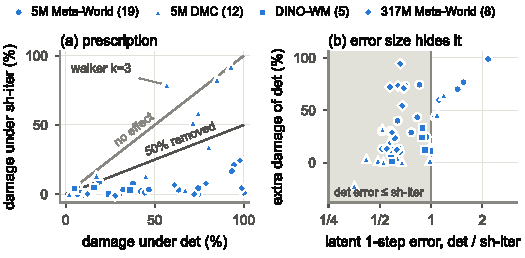
\includegraphics[width=\columnwidth]{figures/fig_damage.pdf}
\caption{Every affected cell. (a) Damage under \shiter vs.\ \dtm (success points on Meta-World and DINO-WM, relative return on DMC); below the dashed line \shiter removes at least half of the damage. (b) \dtm's extra damage against the ratio of the two latent one-step errors: most cells sit in the shaded region, where \dtm's error is the smaller one.}
\label{fig:damage}
\end{figure}

\textbf{Prescription.} \shiter removes at least half of the damage in all 19 affected Meta-World cells (median 95\%) and in 4 of 5 DINO-WM cells, and it is not harmful in any of them (Fig.~\ref{fig:damage}a, Table~\ref{tab:hyp}). The stochastic variants share one per-entry error distribution, yet across the 19 affected Meta-World cells the mean drop is 50.1 points under \shep, 34.9 under \shstep, 29.2 under \ind and 4.0 under \shiter, against 44.6 under \dtm; \detshift, which keeps round-to-nearest but moves its grid at every call, also loses only 4.0. The weakest Meta-World cell keeps 47\% of the damage (window-open, 4 bits), and the DINO-WM exception is PushT at 5 bits, where \dtm's damage is only 5 points. On the 317M multi-task model, which needs no change to the method, \shiter removes 75--104\% of the damage in all 8 tasks (e.g.\ mw-peg-insert-side: 98.9 points lost under \dtm, 4.4 under \shiter), and the 95\% interval of $D_{\shiter}-D_{\dtm}$ lies below zero in every task. The primary bit widths at 317M (3--5) are close to those at 5M (3--4), so the larger model is not more robust to rounding.

\textbf{Where it helps less.} On DMC, \shiter removes half of the damage in only 5 of 12 cells and is harmful on walker at 3 bits (78.9\% of return lost vs.\ 56.9\% under \dtm). A rule added after the first stage and tested on new seeds explains where it helps: the persistent share of \dtm's favorable error (drift over OEI) is 0.33--0.52 on DMC and 0.54--0.73 on Meta-World, and across the 12 TD-MPC2 tasks it predicts the damage removed (Spearman 0.83, new seeds). The two DMC tasks with the smallest persistent share are the two where \shiter fails.

\section{Mechanism}
\label{sec:mech}

\textbf{Drift.} Under \dtm the population-mean error drifts in the favorable direction in all four mechanism tasks at their primary bit widths. \shiter keeps at most 24\% of that drift (0.10, 0.24, 0.03 and $-0.01$ of it), and \detshift, which keeps round-to-nearest but moves the grid at every call, keeps at most 15\%. The positive controls isolate persistence: holding the \emph{same} shared dither fixed for a control step (\shstep) or an episode (\shep) brings back 70--130\% of \dtm's drift in the three TD-MPC2 tasks (Fig.~\ref{fig:mech}a). Error size and sharing are equal across these variants; only persistence differs. On PushT the full-size fixed table did not reproduce the drift (ratio 0.01); there a fixed dither was exploited only when we made its table of offsets coarse, as below.

\begin{figure*}[t]
\centering
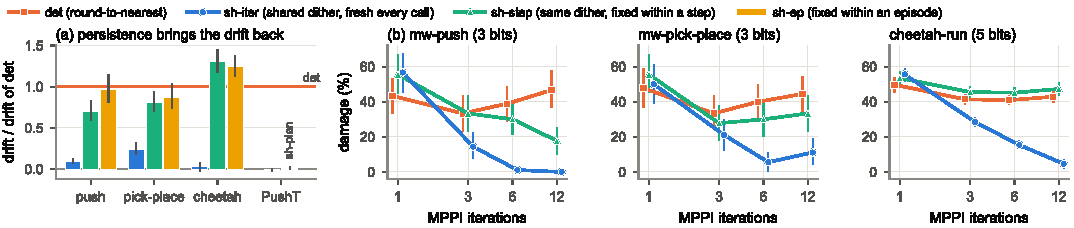
\includegraphics[width=\textwidth]{figures/fig_mechanism.pdf}
\caption{Mechanism. (a) Favorable drift of the population-mean error kept by each variant, relative to \dtm (TD-MPC2 at its primary bit width; PushT at 4 bits, where \shstep and \shep coincide as sh-plan); bars show 95\% bootstrap intervals. (b) Damage vs.\ MPPI iterations (TD-MPC2, 90 paired episodes per point, 95\% intervals). Fresh dither needs iterations to help; \dtm does not improve with them.}
\label{fig:mech}
\end{figure*}

\textbf{Iterations, candidates and table size.} The fix needs an iterating planner. With one MPPI iteration \shiter is no better than \dtm; at 12 iterations its damage is 0--11\% while \dtm's stays at 43--47\% and \shstep's at 18--47\% (Fig.~\ref{fig:mech}b). With the number of elites fixed, \dtm's exploitation $|\mathrm{OEI}|$ and damage grow with the number of candidates in three of four tasks, the dose-response expected from the optimizer's curse~\cite{smith2006curse}. A fixed dither drawn from a table of $N_{\mathrm{eff}}$ independent offsets hurts less as the table grows (five of six tasks, three of them exactly at the threshold), and in an exploratory Wall cell (3 bits) a single offset per layer collapsed planning (+37 points).

\textbf{Theory.} For a planner that averages fresh unbiased noise, the expected drift is zero. A persistent error field instead pulls the population toward the minimizer of the smoothed model cost, the bias of sample-average approximation~\cite{kleywegt2002saa}. The selection and drift terms we derived matched 922k simulated MPPI and CEM runs (fitted slopes 0.92--1.05) and predicted, before the first stage was analyzed, that the OEI would be negative even under fresh noise, because the last iteration's pick benefits from the noise it was selected on (the winner's curse). This is why our original OEI tests, H2a and H2b, failed, and why our mechanism claim concerns the drift rather than the OEI.

\section{Deployment: Latency and Number Formats}
\label{sec:deploy}

\textbf{Integer kernels.} A fused Triton kernel (int8 weights, 4- or 8-bit activation codes, shared dither drawn on the GPU) reproduces the fake-quantization results in closed loop, and 8-bit activations cause no damage. Run eagerly at 5M parameters and 512 candidates, it was 18\% slower than FP32: the step is bound by kernel launches, not arithmetic. To map where low bit widths pay off, we timed one control step's world-model rollouts (6 iterations $\times$ 3 horizon steps of dynamics and reward for $N$ candidates, plus the policy trajectories) replayed as a single CUDA graph, as TD-MPC2's compiled planner does. The integer path uses int8 weights (per output channel) and 4-bit activation codes with int8 tensor-core GEMMs; the first layer, whose input $[z,a]$ is not quantized, stays in FP32. On an NVIDIA A40, across 5M--317M parameters and $N\in\{512, 2048, 8192\}$ (10 interleaved rounds per condition), the integer rollout is 1.9--3.3$\times$ faster than FP32 in all 12 cells and 1.19--1.48$\times$ faster than the faster of TF32 and BF16 in 10 of 12 (Fig.~\ref{fig:latency}); shared dither changes latency by $-0.2$ to $+2.1\%$, because one draw per layer and call serves every candidate. The gains are largest at 317M, the size at which the multi-task results of Sec.~\ref{sec:fix} hold. The full planning step, run eagerly with the encoder, policy and eight Q-functions in FP32, gains less: 1.35$\times$ over FP32 and 1.05$\times$ over the fastest float format at 317M. % E8c (pre-cast BF16, full step as one CUDA graph): fill in when the run is verified.

\begin{figure}[t]
\centering
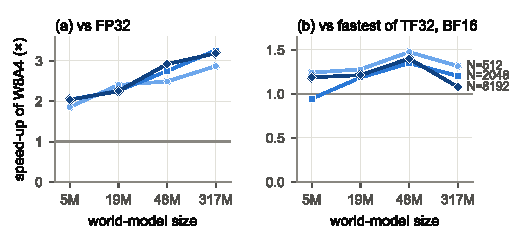
\includegraphics[width=\columnwidth]{figures/fig_latency.pdf}
\caption{Speed-up of the W8A4 integer world model over FP32 (a) and over the faster of TF32 and BF16 (b) for one control step of MPPI rollouts replayed as a CUDA graph (NVIDIA A40; $N$ candidates, 6 iterations, horizon 3). BF16 uses autocast, which converts the weights at every call.}
\label{fig:latency}
\end{figure}

\textbf{FP4 formats mark the boundary.} Recent accelerators execute 4-bit floating point natively; on an RTX 5090, an NVFP4 GEMM at the 317M layer width is up to 5.3$\times$ faster than BF16. We therefore repeated the 5M experiment with the activations in NVFP4~\cite{nvidia2025nvfp4} (blocks of 16 with an E4M3 scale) and MXFP4~\cite{rouhani2023mx} (blocks of 32 with a power-of-two scale), rounding each block to the E2M1 grid either to nearest (\dtm) or stochastically (\shiter). In TD-MPC2, block scaling greatly reduces the damage. \dtm damaged only 2 of 12 tasks under NVFP4 (cheetah-run 9.9\%, walker 1.7\%), short of the three our analysis plan required, and 4 of 12 under MXFP4 (cheetah-run 31.3\%, window-open 10.0 points), against 71.6\% on cheetah-run with a uniform 4-bit grid. Where damage remained, the signature was the same: \dtm's latent one-step error was 0.48--0.63 times that of \shiter in all six damaged cells, and \shiter removed most of the damage in the one damaged Meta-World cell but in only 2 of 5 DMC cells, as with uniform grids. Fine block scaling shrinks the error; dither removes its persistence. The two remedies act on different axes, and in TD-MPC2 the failure we study belongs to coarse grids with a shared scale; quantized VLA policies can still lose success under NVFP4~\cite{park2026qcrl}.

\section{Limitations and Stage 2 Plan}
\label{sec:stage2}

\textbf{Limitations.} The prescription assumes an iterating planner, and on DMC it helps in fewer than half of the affected cells. On top of the best post-training quantization (mostly per-channel ranges), which already removes most of \dtm's damage, the extra gain of \shiter is borderline in TD-MPC2 (10 of 19 cells) and absent in DINO-WM (1 of 3). We did not combine dither with calibration objectives such as~\cite{anon2026modulemse}. Our quantization-aware-training baseline was weak, so we draw no conclusion about training. The 317M results come from one checkpoint, the latency map from one GPU type with the first layer in FP32, and the FP4 results from fake quantization of the 5M models. We have no physical-robot experiments.

\textbf{Proposed Extension Charter.} As in Table~\ref{tab:hyp}, each item would have its hypotheses, thresholds and analysis code fixed before its data.
\begin{enumerate}
\item \emph{A diagnostic that sees the damage.} The latent one-step error misses \dtm's damage, while the one-step reward error separated \dtm in every affected Meta-World cell (an observation made after the fact). We will test on new tasks and seeds whether the correlation of rounding error across hidden units, which a scalar output such as the reward sums up, predicts \dtm's damage within a bit width, and whether a reward-error check run before deployment flags the damaging configurations.
\item \emph{Integer kernels for DINO-WM.} We will port the integer path to the DINO-WM predictor and test whether closed-loop damage and repair match fake quantization in the affected cells, with the same latency budget for dither ($\le$5\%).
\item \emph{The whole planning step.} We will time the complete MPPI step (encoder, policy, Q-ensemble, sampling and selection) captured as one CUDA graph, against FP32, TF32 and BF16 with pre-converted weights, and relate the speed-up to the control rate it allows.
\item \emph{Embedded and FP4 hardware.} We will repeat the latency map on an NVIDIA Jetson module and, with fused quantization kernels, for NVFP4 on a Blackwell GPU, including the cost of drawing dither.
\end{enumerate}
The negative results above (DMC, the combination with strong post-training quantization, planners with few iterations) stay in scope as boundaries to report, not as targets to tune away.

\bibliographystyle{plainnat}
\bibliography{refs}

\end{document}
